\section{Results and Evaluation}
This section presents the results of our experiments across exploratory data analysis, spatial and temporal regression, future forecasting, unmonitored location estimation, and AQI classification.

\subsection{Exploratory Data and Spatial Trends}
Fig. \ref{fig:city_and_month}a displays the mean $\text{PM}_{2.5}$ AQI reading for each monitoring city. Inland centers such as Bloemfontein (76.88), Johannesburg (75.60), Pretoria (75.43), and Vereeniging (71.38) show higher pollution levels than coastal towns such as Richards Bay (24.55), Worcester (28.60), and Cape Town (33.56).

Fig. \ref{fig:city_and_month}b displays the monthly average $\text{PM}_{2.5}$ profile with a 95\% confidence band. Pollution peaks during the southern hemisphere winter (June and July) and declines during summer months (December to February). Thermal inversions may trap emissions during colder months, though this was not tested here.

\begin{figure}[htbp]
\centering
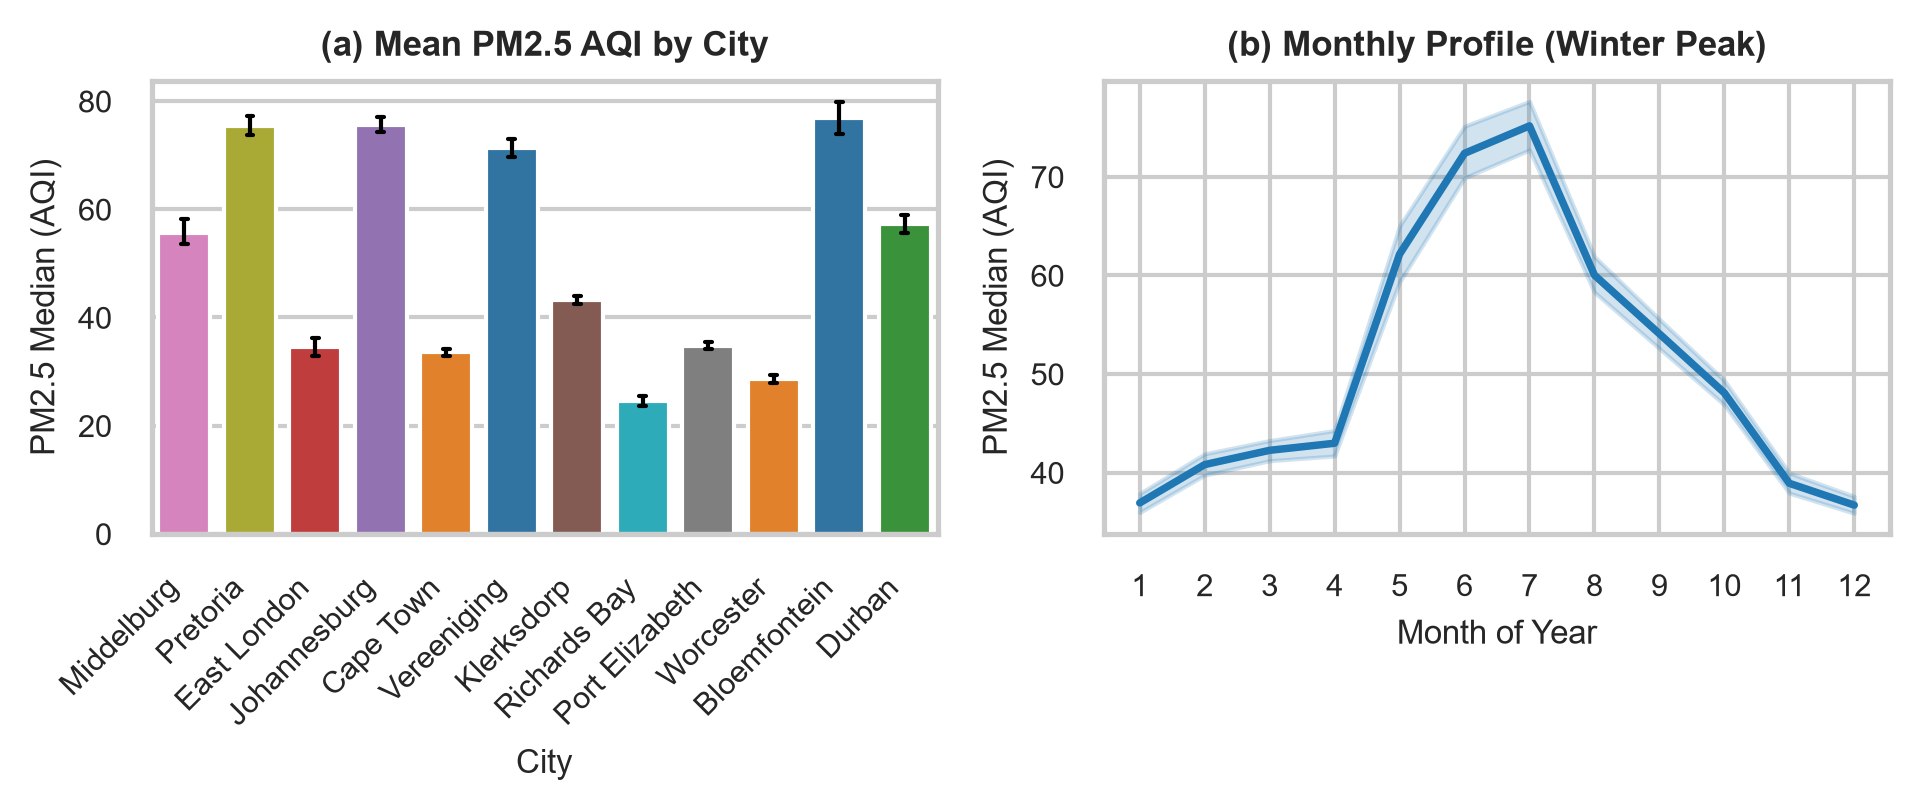
\includegraphics[width=\linewidth]{figures/figure2_city_and_month_pm25.png}
\caption{Observed PM2.5 AQI patterns: (a) Mean level by city with error bars, and (b) Monthly average profile showing winter peak.}
\label{fig:city_and_month}
\end{figure}

\subsection{Spatial and Temporal Regression Cross-Validation}
In the primary 5-fold spatial cross-validation, the test cities for each fold were: Fold 0 (Pretoria, Vereeniging; 10 train, 2 test), Fold 1 (Bloemfontein, Port Elizabeth; 10 train, 2 test), Fold 2 (Cape Town, Middelburg, Richards Bay; 9 train, 3 test), Fold 3 (Durban, East London, Johannesburg; 9 train, 3 test), and Fold 4 (Klerksdorp, Worcester; 10 train, 2 test). Our training city counts per fold are 10, 10, 9, 9, and 10, whereas the base paper reported 9, 9, 10, 10, and 10. While both configurations match as an unordered multiset, the fold assignments occur in a different sequence, and we do not claim the same fold order.

Across the five folds, CatBoost achieved a mean fold RMSE of 28.863, and XGBoost achieved a mean fold RMSE of 28.576. In our run, XGBoost had the slightly lower average fold error. Fold 1 produced the highest error (CatBoost RMSE 34.815, XGBoost RMSE 36.453), while Fold 4 produced the lowest error (CatBoost RMSE 19.259, XGBoost RMSE 14.641).

In the secondary per-city \texttt{TimeSeriesSplit} cross-validation (5 splits, 150-day test window, 24-day gap), CatBoost achieved an overall average RMSE of 19.893 across the twelve cities, and XGBoost achieved 20.265. Evaluating within individual stations yields lower error than spatial holdouts because the model calibrates to station-specific baseline levels. Klerksdorp showed a very low RMSE (6.783 for CatBoost), which is partly because its sparse data (only 629 raw readings) meant that most dates were filled with the constant city mean.

\subsection{Temporal Date-Split Evaluation}
Table \ref{tab:datesplit_overall} presents the holdout evaluation for models trained before January 1, 2022 and evaluated on the 3,981 observations from 2022. Overall, CatBoost attained an RMSE of 26.218 (MAE 17.916) and XGBoost attained an RMSE of 26.229 (MAE 17.470). Across individual cities, test performance showed a wide spread, ranging from 7.927 RMSE in Klerksdorp (best) to 50.410 RMSE in East London (worst). We record that this evaluation is a historical date split rather than an autoregressive multi-step forecast.

\begin{table}[htbp]
\centering
\small
\caption{Temporal Date-Split Overall Evaluation (Train $<$ 2022-01-01, Test $\ge$ 2022-01-01)}
\label{tab:datesplit_overall}
\begin{tabular}{lccc}
\toprule
Model & Test Records & RMSE & MAE \\ \midrule
CatBoost & 3,981 & 26.218 & 17.916 \\
XGBoost & 3,981 & 26.229 & 17.470 \\
\bottomrule
\end{tabular}

\end{table}

CatBoost tends to under-predict acute peaks above about 100 AQI, as shown in Fig.~\ref{fig:catboost_johannesburg}.

\begin{figure}[htbp]
\centering
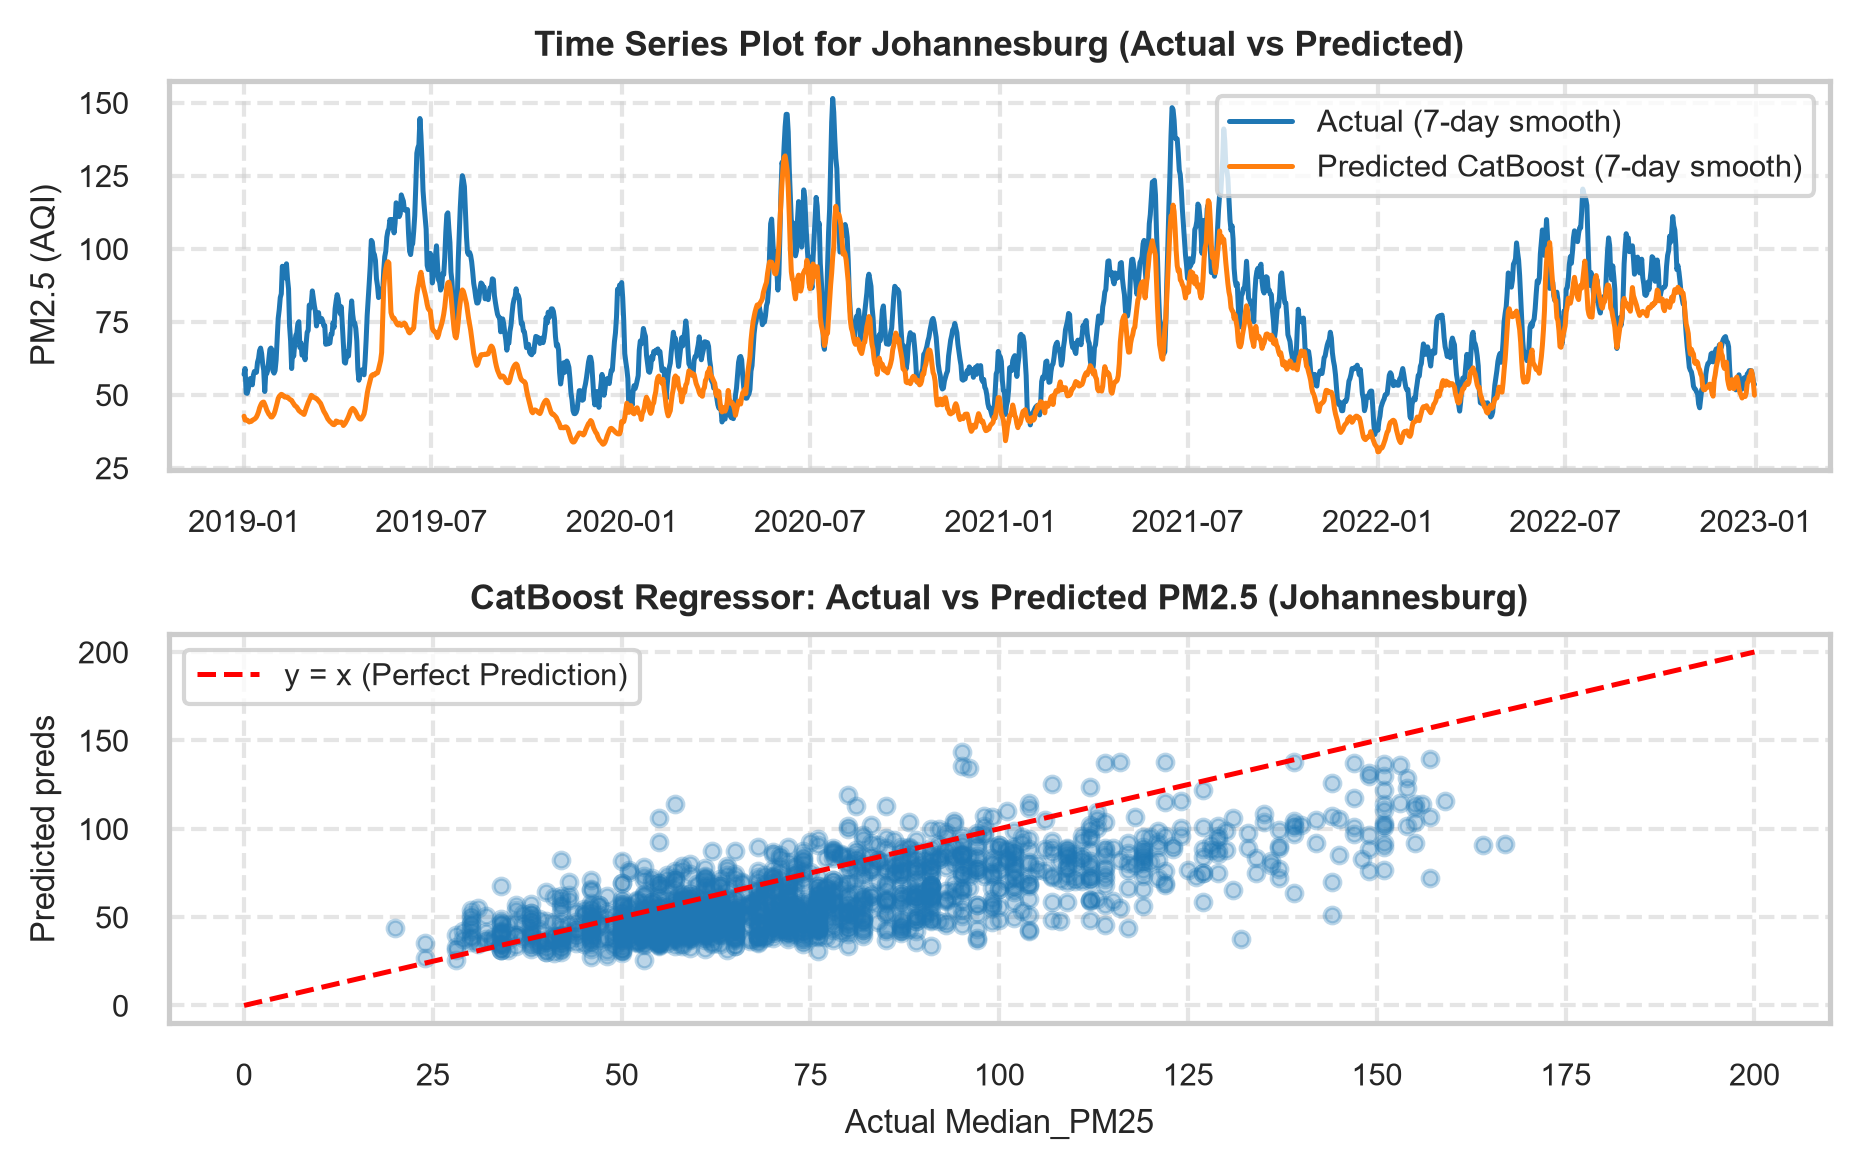
\includegraphics[width=0.88\linewidth,height=5.2cm,keepaspectratio]{figures/figure7_catboost_johannesburg.png}
\caption{CatBoost regression performance on Johannesburg: (top) 7-day smoothed actual versus predicted time series; (bottom) scatter plot with ideal $y=x$ reference line.}
\label{fig:catboost_johannesburg}
\end{figure}

\subsection{Spatial Estimation for Unmonitored Municipalities}
The base paper selected CatBoost for unmonitored predictions; in our implementation, we used XGBoost because it achieved the lower mean fold RMSE in our spatial cross-validation. To evaluate purely spatial interpolation without lagged variables, we computed Leave-One-City-Out (LOCO) cross-validation across all twelve monitored stations. The average LOCO RMSE was 26.522 (MAE 18.363), with the highest errors occurring in Bloemfontein (58.881) and Middelburg (41.407).

Table \ref{tab:unmonitored_predictions} reports the predicted daily mean $\text{PM}_{2.5}$ AQI values for the six unmonitored municipalities during 2022. We treat this experiment as an approximation because the base paper mentioned incorporating Sentinel-5P satellite observations without providing scripts, column products, or processing details. In our implementation, Mahikeng is predicted at 75.887, Lebowakgomo at 51.610, and Kimberley, Kuruman, Upington, and Vryburg all predict 52.141. Because the model relies solely on latitude and longitude coordinates, tree partition splits place all four interior plateau towns into the exact same leaf partition.

\begin{table}[htbp]
\centering
\small
\caption{Predicted 2022 Annual Mean PM2.5 AQI for Unmonitored Municipalities}
\label{tab:unmonitored_predictions}
\begin{tabular}{lccc}
\toprule
City & Latitude & Longitude & Mean Predicted PM2.5 \\ \midrule
Kimberley & -28.7282 & 24.7499 & 52.141 \\
Kuruman & -27.4524 & 23.4327 & 52.141 \\
Lebowakgomo & -24.2000 & 29.5000 & 51.610 \\
Mahikeng & -25.8560 & 25.6403 & 75.887 \\
Upington & -28.4478 & 21.2561 & 52.141 \\
Vryburg & -26.9550 & 24.7280 & 52.141 \\
\bottomrule
\end{tabular}

\end{table}

\subsection{Future Forecasting and Holdout Check}
Figure \ref{fig:future_forecast} displays the two-column by six-row grid of recursive daily forecasts for all twelve cities from November 26, 2022 to December 31, 2023. At each forecast step, simulated predictions updated subsequent lag features. In the resulting trajectories, East London (predicting a maximum of 244.07) and Middelburg (predicting a maximum of 414.90) exhibit unstable spikes, likely due to outlier historical lag values being fed back recursively.

We checked forecast performance against actual sensor readings from November 26 to December 31, 2022. Cape Town, East London, and Richards Bay had stopped reporting earlier in 2022, so their forecasts could not be evaluated. For the nine available cities, the simple average holdout RMSE was 15.771 (MAE 12.751).

\begin{figure}[htbp]
\centering
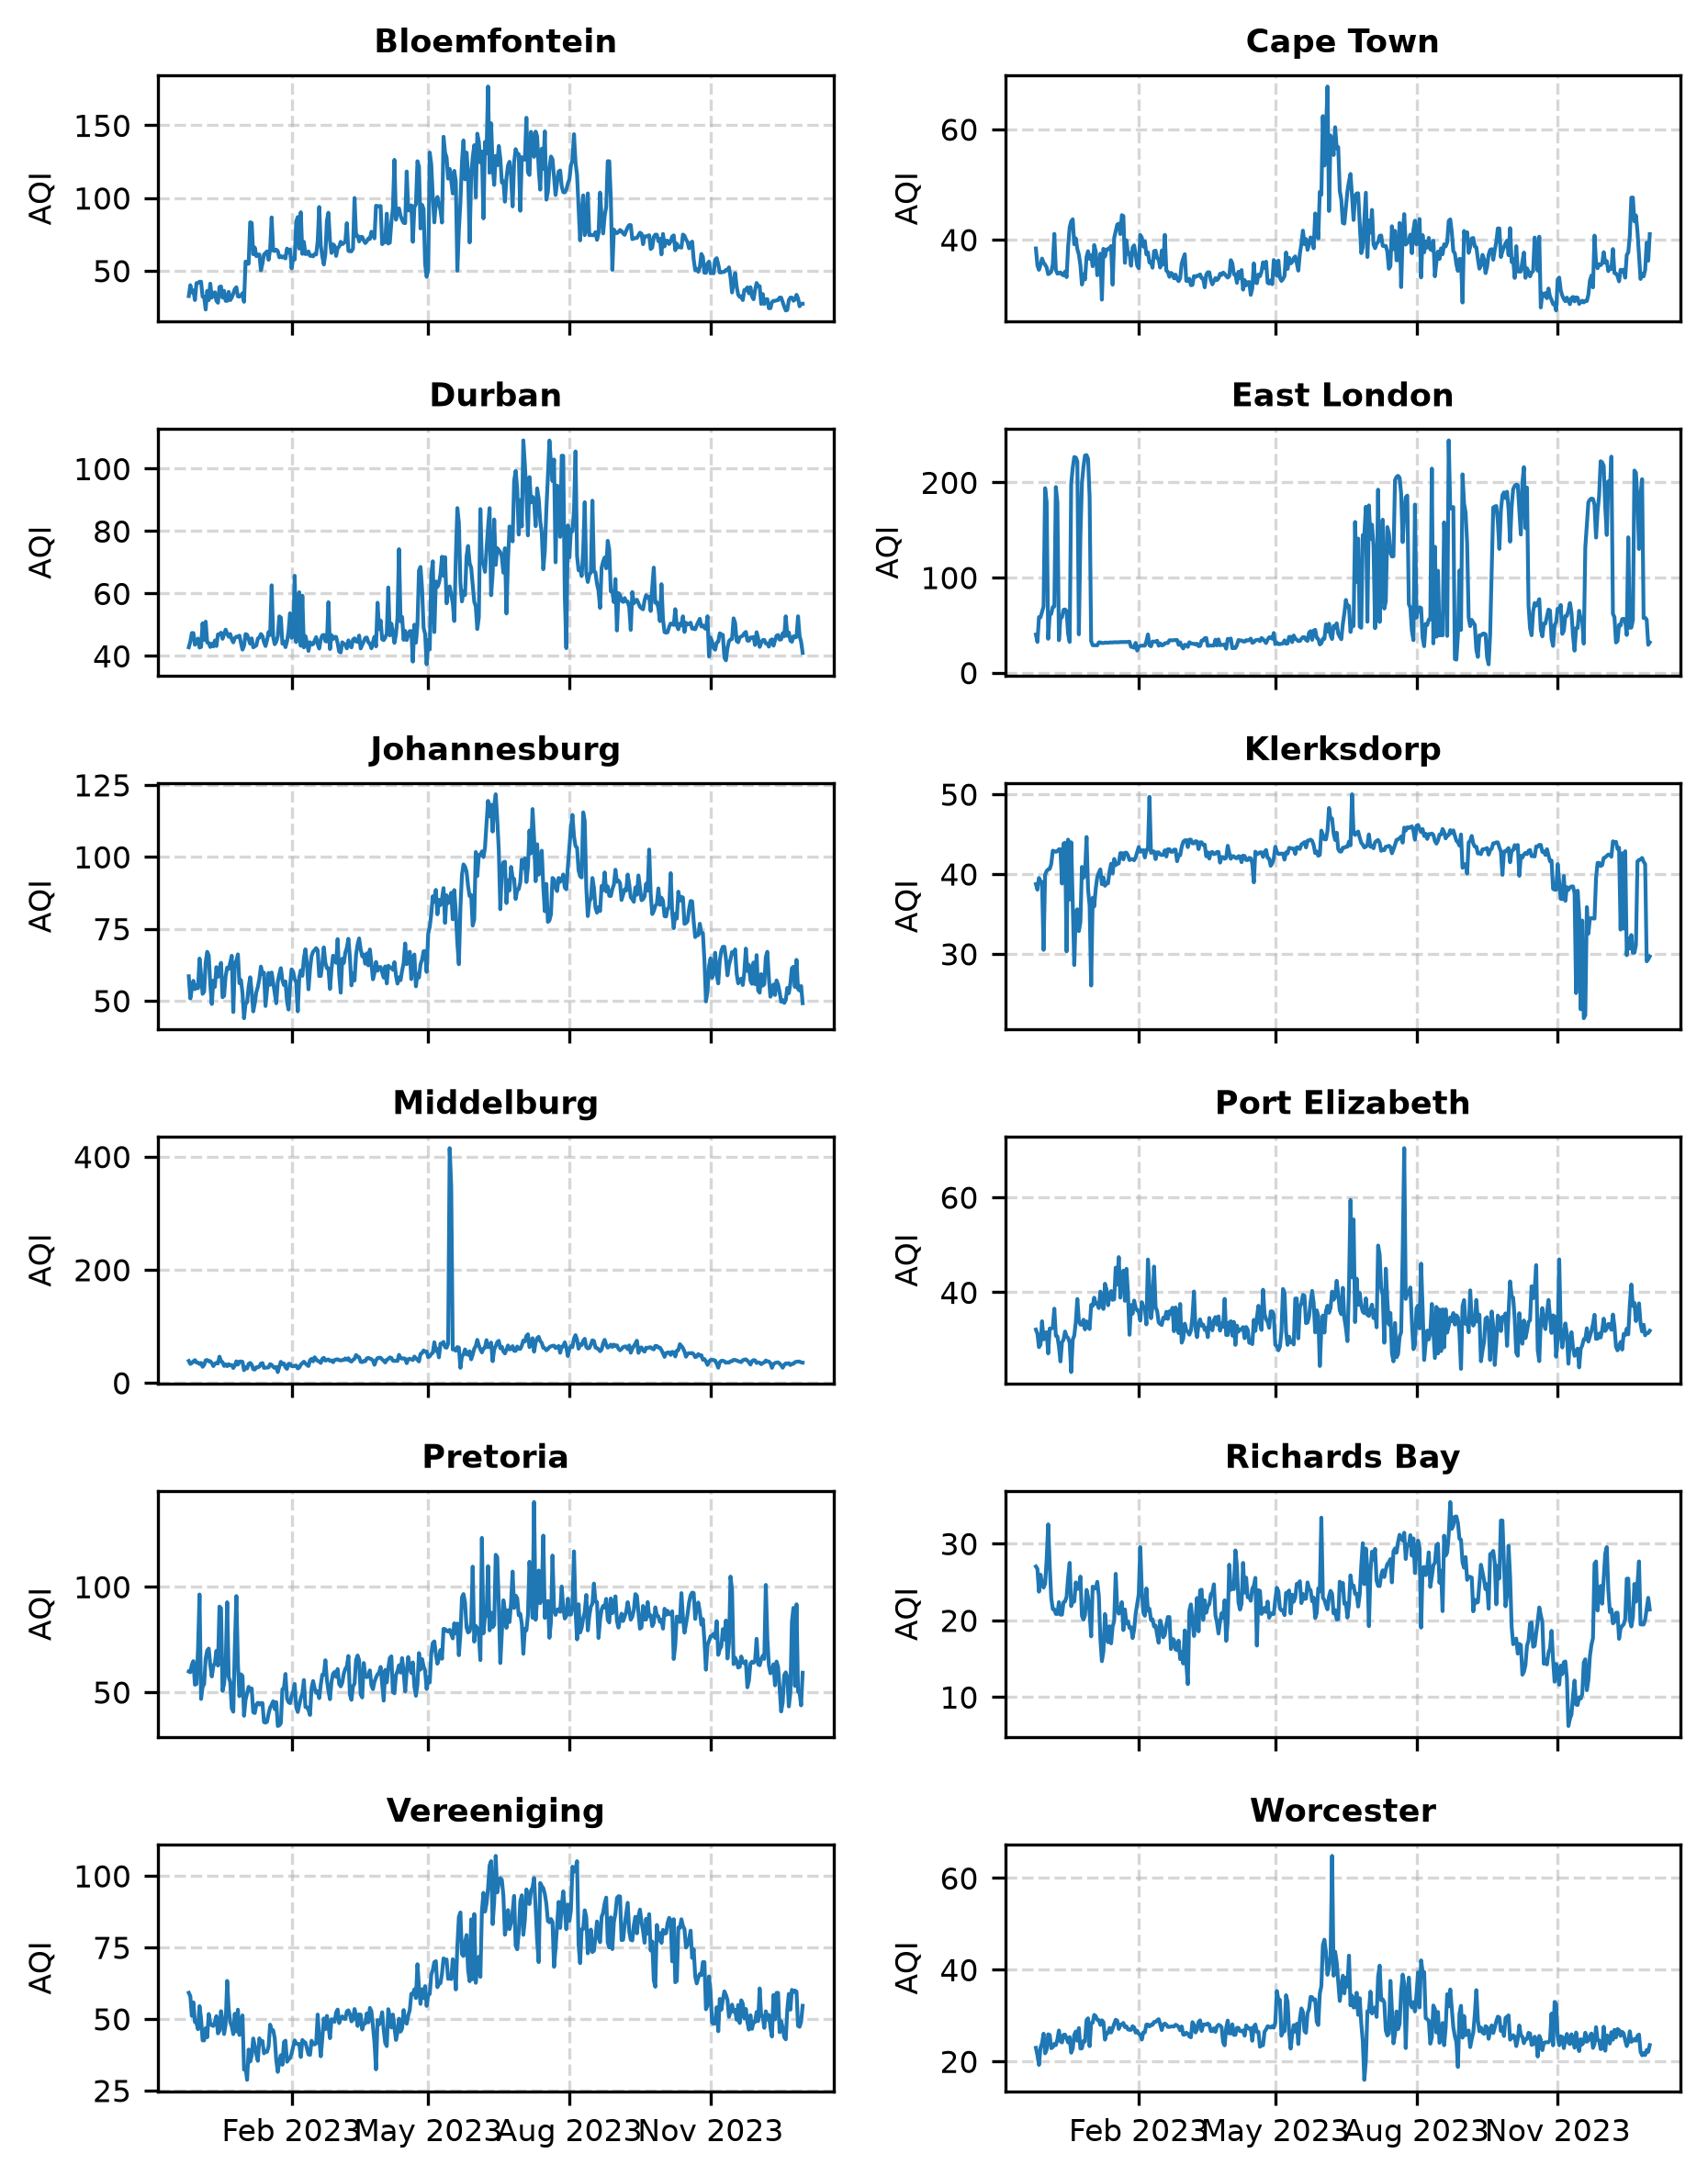
\includegraphics[width=0.85\linewidth,height=7.2cm,keepaspectratio]{figures/figure13_future_forecast_grid.png}
\caption{Recursive daily future PM2.5 AQI forecasts for all twelve cities from November 26, 2022 to December 31, 2023 in a two-column by six-row layout.}
\label{fig:future_forecast}
\end{figure}

\subsection{Air Quality Index Classification}
Table \ref{tab:aqi_classification} summarizes the performance of the five classifiers on the 30\% holdout partition (4,976 samples) and compares accuracy with the base paper. All five models achieved accuracies between 98.834\% and 99.960\%. Random Forest and Decision Tree achieved the highest accuracy (99.960\%), followed by KNN (99.940\%), Logistic Regression (99.900\%), and SVM (98.834\%). In comparison with the paper's Figure 14 macro values (Random Forest 1.00/1.00/1.00, Decision Tree 1.00/1.00/1.00, SVM 0.99/0.99/0.99, KNN 0.82/0.83/0.83, Logistic Regression 0.80/0.77/0.78), our macro metrics show a gap primarily in sensitivity and F1. The gap comes from class 5 (paper test set has 1 Hazardous sample, ours has 2, none predicted correctly), while classes 0 to 4 have precision and recall at or near 1.0.

\begin{table}[htbp]
\centering
\footnotesize
\renewcommand{\arraystretch}{0.90}
\caption{Air Quality Index Classification Performance and Comparison on 30\% Test Partition}
\label{tab:aqi_classification}
\begin{tabular}{lccccccc}
\toprule
Model & Paper Acc & Our Acc & Sensitivity & Specificity & Macro Prec & Macro F1 & RMSE \\ \midrule
Random Forest & 100.000\% & 99.960\% & 0.8333 & 0.9999 & 0.8167 & 0.8246 & 0.020048 \\
Logistic Regression & 98.957\% & 99.900\% & 0.8316 & 0.9998 & 0.8122 & 0.8214 & 0.031699 \\
SVM & 98.881\% & 98.834\% & 0.8237 & 0.9957 & 0.8026 & 0.8124 & 0.107963 \\
KNN & 99.986\% & 99.940\% & 0.8241 & 0.9999 & 0.8143 & 0.8191 & 0.024554 \\
Decision Tree & 100.000\% & 99.960\% & 0.8333 & 0.9999 & 0.8167 & 0.8246 & 0.020048 \\
\bottomrule
\end{tabular}

\end{table}

Fig. \ref{fig:confusion_matrices} displays the confusion matrices for all five classifiers. In our results, macro Sensitivity is about 0.82 to 0.83 (0.8333 for Random Forest and Decision Tree, 0.8316 for Logistic Regression, 0.8241 for KNN, and 0.8237 for SVM), whereas the base paper reported 1.0. A detailed inspection explains this difference: the test set has only 2 samples of Class 5 (Hazardous), both having $\text{PM}_{2.5}\text{ AQI} = 999.0$, while the training partition contains 0 samples of Class 5 (out of 11,609 training instances), so no classifier could learn this category. Consequently, all five classifiers predicted Class 4 (the highest class seen during training) for both Class 5 test samples, producing zero recall for Class 5. Other misclassifications were minimal: Random Forest and Decision Tree made only the two Class 5 errors, KNN made 3 (including 1 Class 4 sample at 203.0 predicted as Class 3), and Logistic Regression made 5 (3 Class 2 samples at 150.0 predicted as Class 3, plus the two Class 5 errors). SVM made 58 errors: 48 samples of true Class 1 were predicted as Class 0 at $\text{PM}_{2.5} = 51.0$, 8 samples of true Class 2 were predicted as Class 3 at $\text{PM}_{2.5} \in [149.0, 150.0]$, and 2 samples of true Class 5 were predicted as Class 4 at $\text{PM}_{2.5} = 999.0$. Thus, 56 of the 58 SVM errors occurred directly at category boundaries (51.0 and 149.0 to 150.0). In the demo test (input 125.55), all five classifiers returned Class 2 (Unhealthy for Sensitive Groups), matching the paper.

\begin{figure}[htbp]
\centering
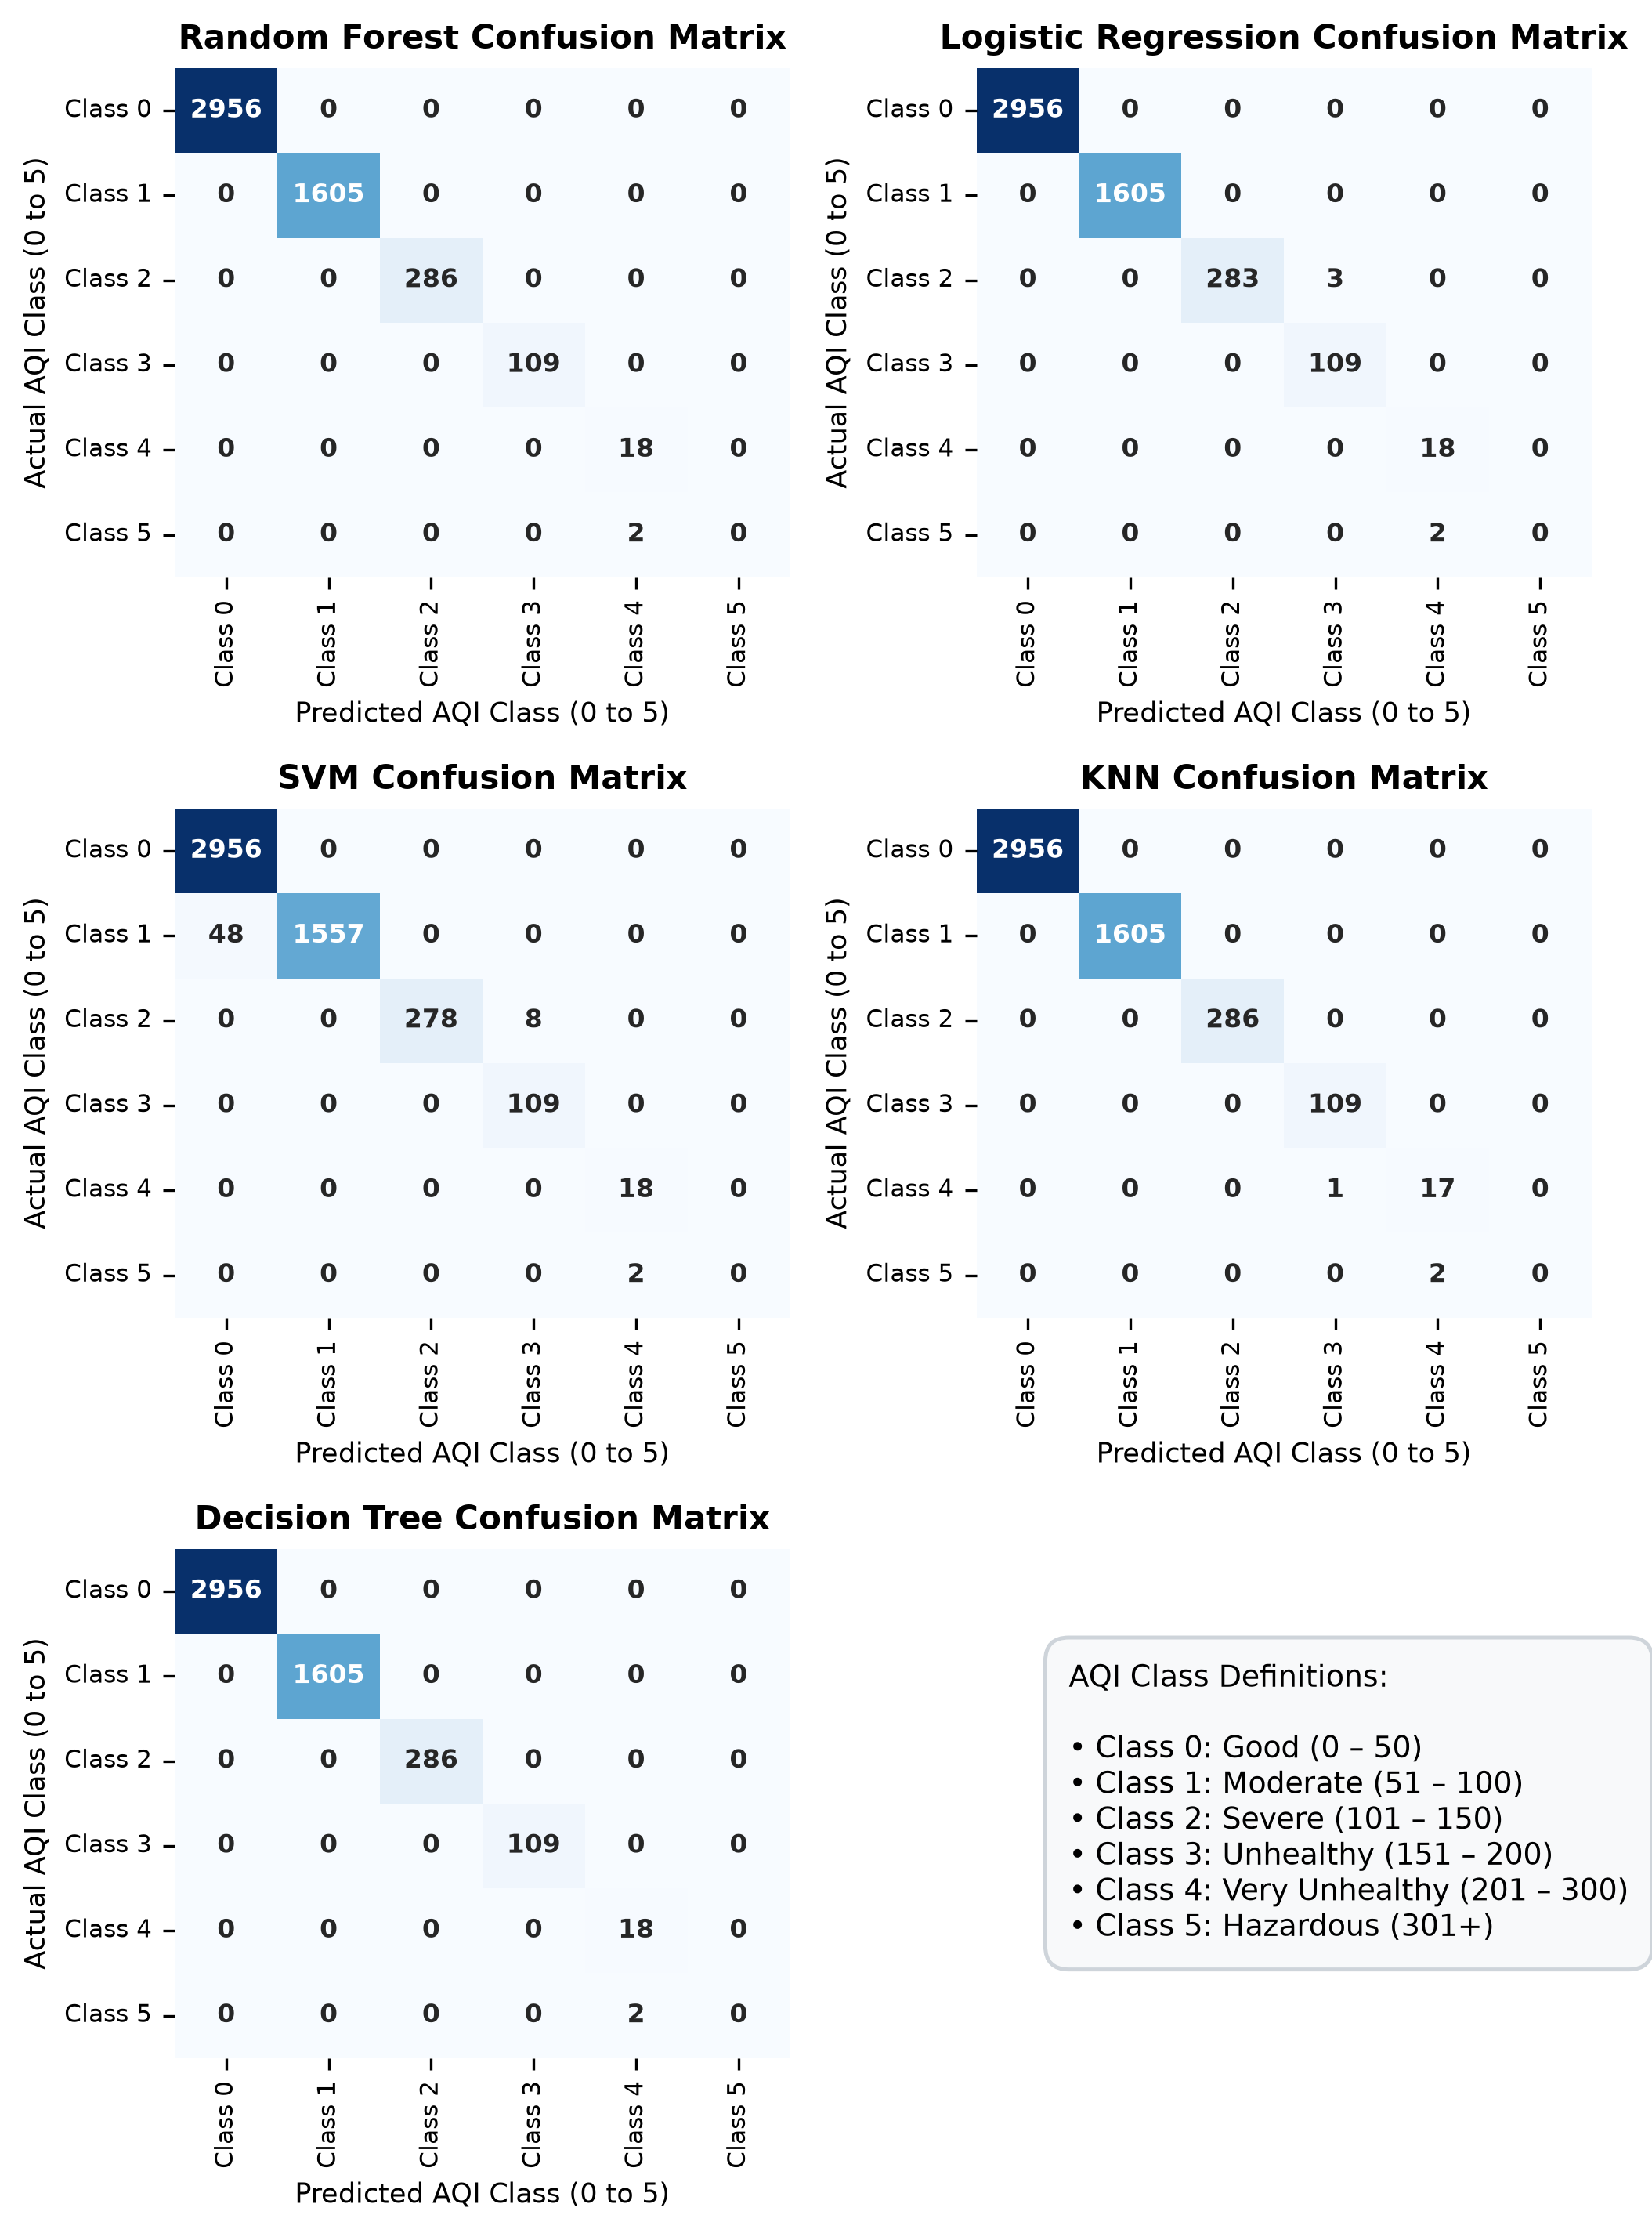
\includegraphics[width=0.85\linewidth,height=7.0cm,keepaspectratio]{figures/figure14_classification_confusion_matrices.png}
\caption{Confusion matrices for the five AQI status classifiers evaluated on 4,976 test samples in a two-column layout with explicit class labels.}
\label{fig:confusion_matrices}
\end{figure}
